\refstepcounter{chapter}
\addcontentsline{toc}{chapter}{INHALTSVERZEIGNIS}

\thispagestyle{coverpage}

\begin{titlepage}
    \thispagestyle{coverpage}

    \vspace*{0cm}

    {\sffamily

        \noindent
        \begin{tabularx}{\textwidth}{X r}
            
\includegraphics[height=1.5cm]{maho-logo.png} &
            {\Huge \textbf{Operator's Manual}} \\
            \multicolumn{2}{l}{\rule{\textwidth}{0.4mm}} \\
            & {\normalsize Nr. 76.34521}
        \end{tabularx}

        \centering
        \vspace{2cm}

        {\fontsize{60pt}{62pt} \bfseries MH400E}\\[1cm]

        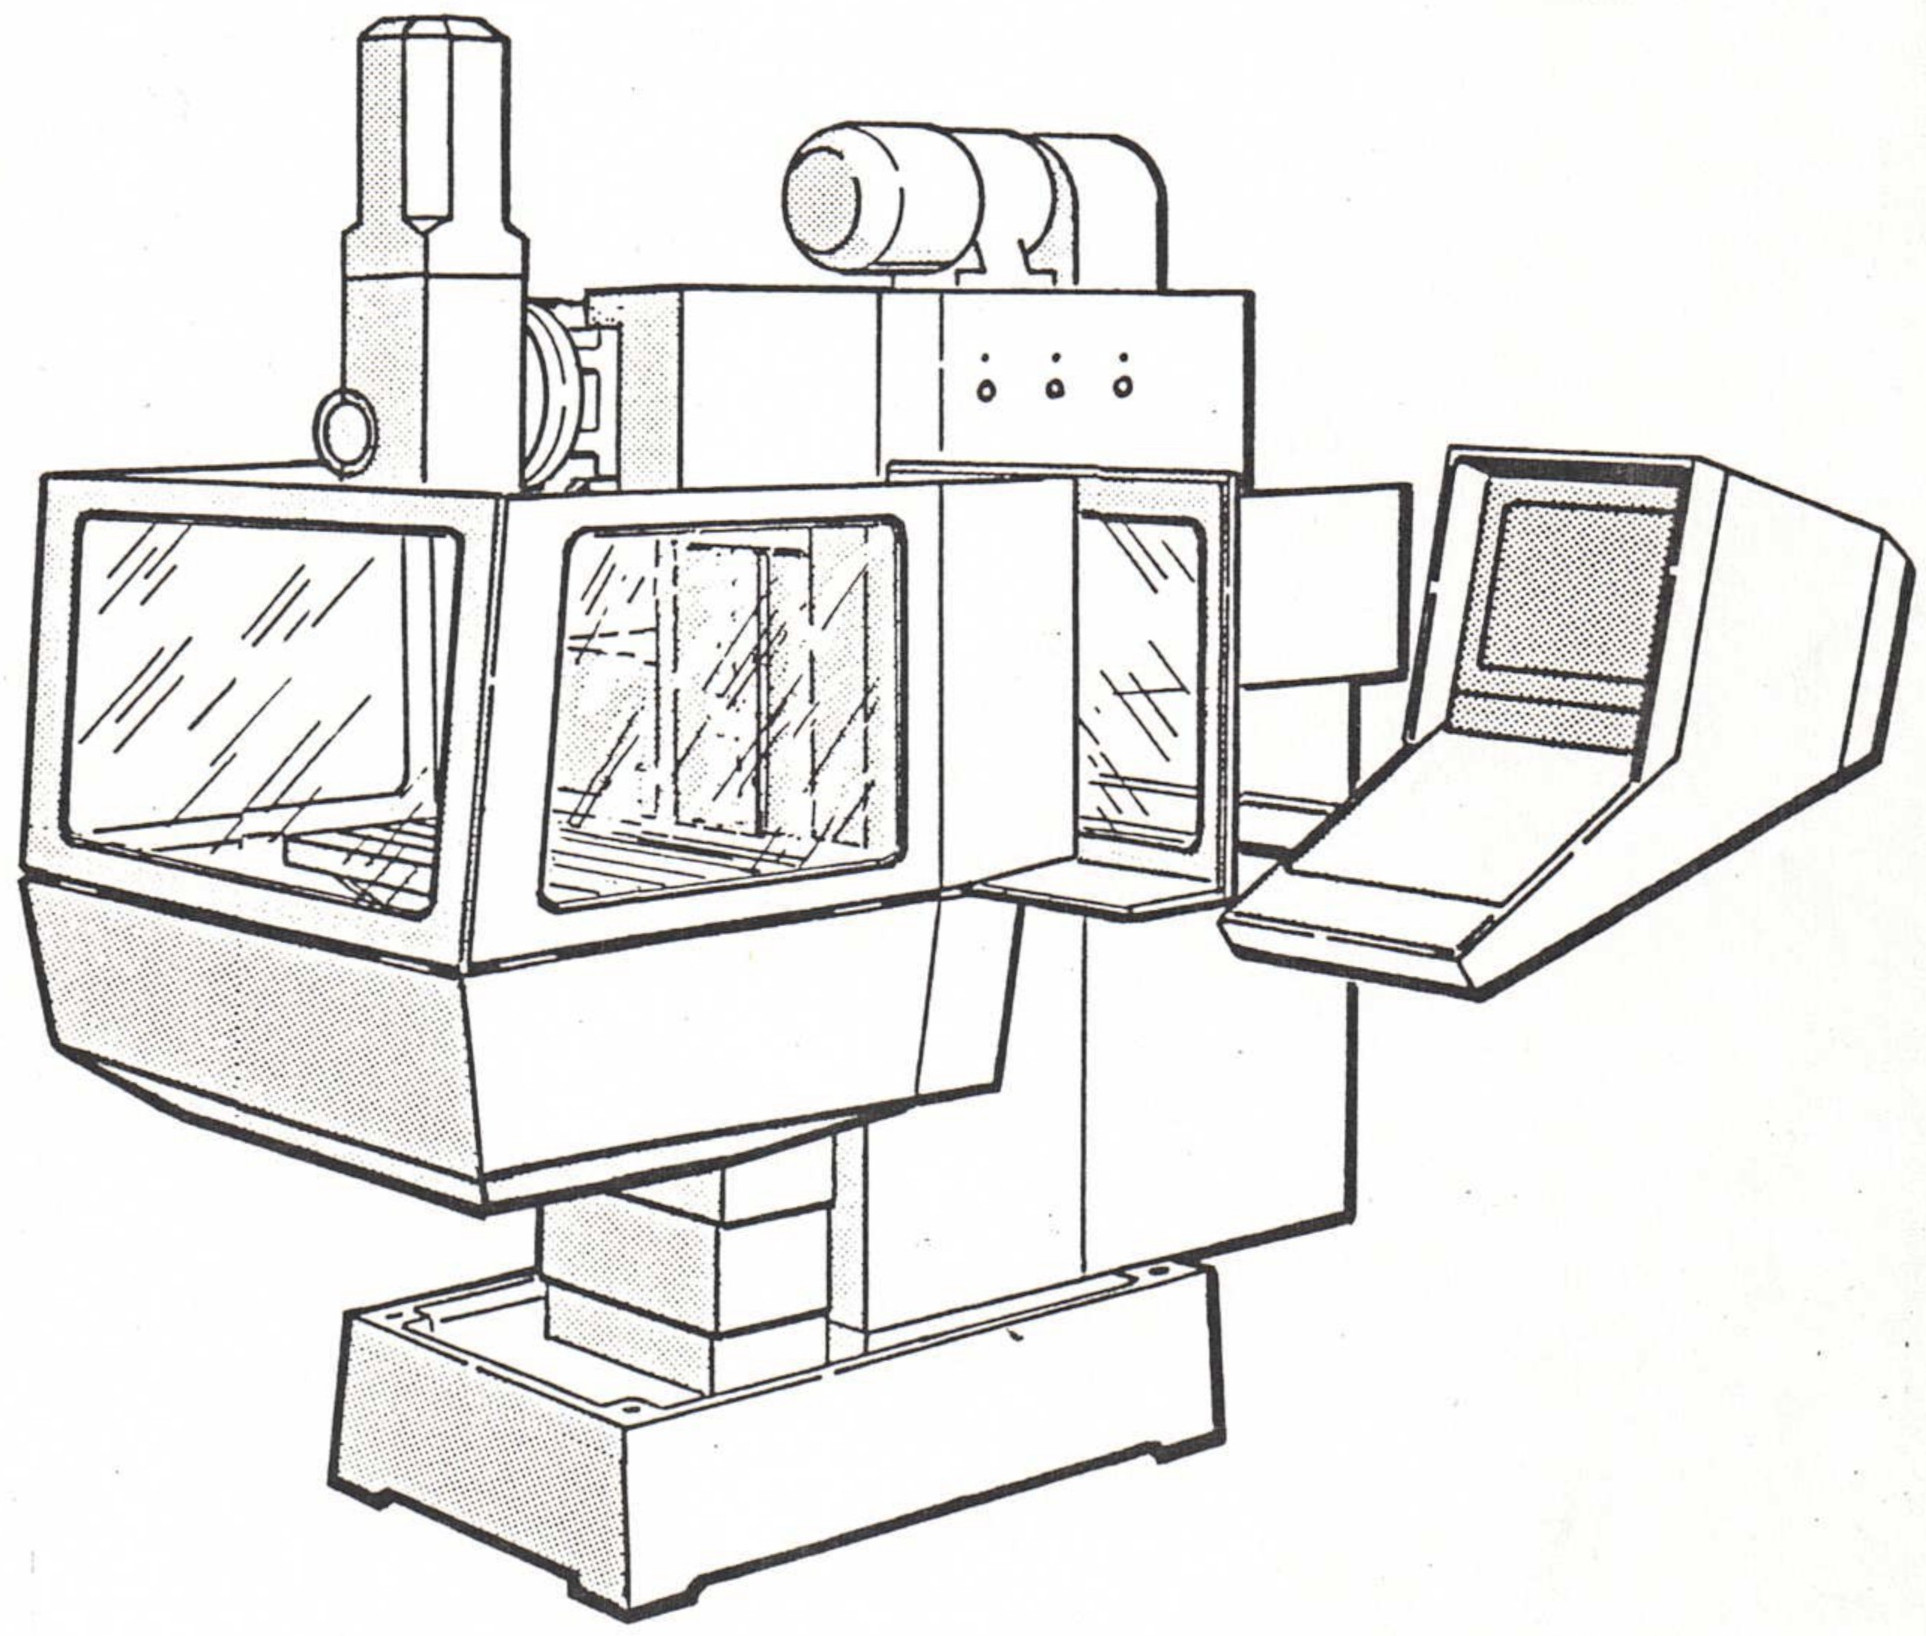
\includegraphics[width=0.9\textwidth]{chapter0/cover-image.jpg} 

        \vfill

         \noindent
         \begin{center}
             \parbox{\textwidth}{\centering {\Huge \textbf{Operation - Maintenance - Repair}}}
         \end{center}
    }
\end{titlepage}

\newpage

\section*{Disclaimer}

This document is an \textbf{unofficial translation} of the original German manual for the Maho MH400E. It has been translated to English to help owners and users of these machines.

\begin{itemize}
    \item This translation is provided \textbf{as-is}, with \textbf{no guarantees regarding accuracy or completeness}.
    \item This document is \textbf{not affiliated with, endorsed by, or approved by DMG-Mori} or any other rights holder.
    \item All trademarks, brand names, and copyrights belong to their respective \\owners.
    \item This document is intended for \textbf{personal and educational use only}. It may \textbf{not be used for commercial purposes}.
    \item If the original rights holder objects to the distribution of this \\translation, the document will be removed upon request.
\end{itemize}

By using this document, you acknowledge that the original manufacturer's documentation remains the \textbf{authoritative source} for technical specifications and procedures. Use this translation at your own risk.

\clearpage % Move to the next page and resume normal styling

\pagestyle{fancy} % Re-enable the default layout

\setsectiontitle{To our customers}
\setcounter{chapter}{0}
\setcounter{section}{0}

This operator's manual contains the essential information required for the proper operation and maintenance of your MAHO machine tool. It belongs in the hands of the operating and maintenance personnel.

The present operator's manual includes the separate operating instructions for CNC 432/10 graphics, the programming instructions for CNC 432 of the control unit, the programming manual for the \enquote{Geometry Package}, and the folder \enquote{Assembly Drawings and Parts Lists}.

Tax-specific details are listed \textbf{only} in the operating manual for CNC 432/10 graphics and should be referenced there.

The machine may only be put into operation after the operating and maintenance personnel have carefully read the operator's manual and have thoroughly\\ familiarized themselves with all details.

Operation and maintenance of the machine must be carried out in accordance with the instructions provided in this operator's manual.

\notebox{NOTE}{\textbf{We assume no liability for damages resulting from failure to follow these instructions or from improper handling.}}

If malfunctions occur that cannot be resolved independently, the cause of the malfunction should be determined using the operator's manual before \\contacting the appropriate MAHO representative or the MAHO company.

This operator's manual is designed to help you complete your machining tasks efficiently. We are confident that the delivered MAHO machine tool will fully meet your expectations. \\[1cm]

\noindent
\textbf{\textcopyright\ Copyright} \\[0.2cm]

This technical manual may \textbf{not}, even in part, be reproduced or made accessible to third parties without the express permission of the publisher.

\newpage

\subsection{Page Numbering}

The pages of this manual are numbered sequentially within each chapter \\according to sections. The page numbers are displayed in the upper right corner and are structured so that the page number follows the section number.

\textbf{EXAMPLE}: \texttt{3.20-3}, means Chapter 3, Section 20, Page 3.

If expansions occur within a section, these are numbered using the page number of the previous page followed by the numbers 1, 2, 3, etc., separated by a period.

\textbf{EXAMPLE}: \texttt{3.20-3.1}, means Chapter 3, Section 20, Page 3, Supplementary Page 1.

Figures and tables are not separately numbered.

The position numbers in the figures refer to the content of the section and can span 2-3 figures.

If positions of a figure are referenced in the text, they are placed within parentheses \texttt{()}.

\subsection{Notices in this Manual}

The following notices are used in this manual:

\notebox{NOTICE}{Applies to technical details that the user must observe.}

\notebox{CAUTION}{Applies to work or operational procedures that must be followed precisely to prevent damage or destruction of the system.}

\notebox{WARNING}{Applies to work or operational procedures that must be followed precisely to prevent hazards to personnel. This also includes \textbf{CAUTION}.}

\subsection{Cross-References}

To avoid redundant descriptions, content-related connections are established in this manual using cross-references.

\textbf{EXAMPLE}:
\begin{quote}
\noindent \hspace{-0.25cm} .... according to instructions .... \\
\hspace{1.3cm} .... see Sheet/Page ....
\end{quote}

\subsection{Location Definition}

The designations front, back, left, right, top, and bottom are based on the perspective from the spindle head looking toward the workpiece.

\setsectiontitle{Table of Contents}
\renewcommand{\arraystretch}{1.3} % Adjust row spacing for readability

\begin{tabularx}{\textwidth}{X r}
    \textbf{\underline{Commissioning the Machine}} & \\ % Main Section (No page number)
    Important Notes \dotfill & 1.01-1 \\
    Transport of the Machine \dotfill & 1.02-1 \\
     & 1.02-2 \\ % No extra &
    Setting Up the Machine \dotfill & 1.03-1 \\
     & 1.03-2 \\
     & 1.03-3 \\
    Setup Plan and Workspace Layout \dotfill & 1.04-1 \\
    Dimensional Drawing of the Machine \dotfill & 1.05-1 \\
    Removal of Rust Protection Agent \dotfill & 1.08-1 \\
    Spindle head oil fill \dotfill & 1.09-1 \\
    Connecting to the Electrical Network \dotfill & 1.10-1 \\
    Commissioning Checklist \dotfill & 1.11-1 \\[0.5cm]

    \textbf{\underline{General Description of the Machine}} & \\ % Main Section
    Technical Data \dotfill & 2.01-1 \\
     & 2.01-2 \\
    Machine Overview \dotfill & 2.02-1 \\
    Component Identification \dotfill & 2.02-2 \\
     & 2.02-3 \\
     & 2.02-4 \\
     & 2.02-5 \\
     & 2.02-6 \\
     & 2.02-7 \\
     & 2.02-8 \\
    Motion Directions \dotfill & 2.03-1 \\
    Control Station \dotfill & 2.04-1 \\
     & 2.04-2 \\
    Hand Control Panel \dotfill & 2.04-5 \\
    Gear Train Schematic \dotfill & 2.10-1 \\
    Main Gearbox \dotfill & 2.10-2 \\[0.5cm]

    \textbf{\underline{Machine Operation}} & \\
    Functional Testing - Trial Run \dotfill & 3.01-1 \\
     & 3.01-2 \\[0.5cm]
\end{tabularx}

\newpage

\begin{tabularx}{\textwidth}{X r}
    Manual Spindle Speed Selection \dotfill & 3.03-2 \\
    Horizontal Working Spindle \dotfill & 3.04-1 \\
    Horizontal Milling with Counter Holder \dotfill & 3.05-1 \\
    Horizontal to Vertical Conversion \dotfill & 3.07-1 \\
    Vertical to Horizontal Conversion \dotfill & 3.08-1 \\
    Vertical Milling Head without Quill Feed \dotfill & 3.09-1 \\
    Automatic Tool Clamping \dotfill & 3.12-1 \\
    Reworking of Standard Tool Shafts \dotfill & 3.13-1 \\
    Tool Shaft According to DIN 69871 \dotfill & 3.13-3 \\
    Manual Adjustment of the Machine Slide \dotfill & 3.15-2 \\
    Hydraulic Plan and Equipment List \dotfill & 3.18-1 \\
    Hydraulic System \dotfill & 3.18-3 \\
    Automatic Central Lubrication System \dotfill & 3.20-1 \\
    Equipment List - Automatic Central Lubrication \dotfill & 3.20-2 \\
    Automatic Central Lubrication \dotfill & 3.20-3 \\
     & 3.20-4 \\
     & 3.20-5 \\
    Coolant System \dotfill & 3.22-1 \\
    Splash Protection \dotfill & 3.24-1 \\[0.5cm]

    \textbf{\underline{Worktables}} & \\
    Fixed Angle Table \dotfill & 4.01-1 \\
     & 4.01-2 \\
    Universal Rotary Table \dotfill & 4.03-1 \\
     & 4.03-2 \\
     & 4.03-3 \\
     & 4.03-4 \\
     & 4.03-5 \\
     Angle Adjustment Display for B-Axis \dotfill & 4.04-1 \\[0.5cm]
\end{tabularx}

\newpage

\begin{tabularx}{\textwidth}{X r}
    \textbf{\underline{CNC Control}} & \\ % Main Section (No page number)
    Linear Measurement Systems and Display Units \dotfill & 5.01-1 \\
    Machine Constants CNC 432 \dotfill & E3.21741C \\
     & E3.21742C \\
     & E3.21743C \\
     & E3.21744C \\
     & E3.24628C \\
     & E3.24629C \\
     & E3.24630C \\
    Error List CNC 432 \dotfill & E3.22870C \\
     & E3.22871C \\
     & E3.22872C \\
     & E3.25024C \\
    Operating Manual CNC 432/Graphics \dotfill & 76.00471 \\
    Geometry Package for CNC 432/Graphics \dotfill & 76.00461 \\
    Programming Manual CNC 432 \dotfill & 76.00211 \\[0.5cm]

    \textbf{\underline{Accessories}} & \\ % Main Section
    High-Speed Milling Spindle \dotfill & 6.02-1 \\
    Dot-Matrix Printer ZIP 30 (Separate Manual) \\[0.5cm] % No page number

    \textbf{\underline{Maintenance}} & \\ % Main Section
    Important Notes \dotfill & 7.01-1 \\
    Machine Lubrication Plan \dotfill & 7.02-1 \\
    Lubrication Schedule \dotfill & 7.03-1 \\
    Lubricant Recommendations \dotfill & 7.06-1 \\
     & 7.06-2 \\
    Coolants \dotfill & 7.07-1 \\
     & 7.07-2 \\
     & 7.07-3 \\
     & 7.07-4 \\[0.5cm]
\end{tabularx}

\newpage

\begin{tabularx}{\textwidth}{X r}
    Removing the Machine Covers \dotfill & 7.10-1 \\
    Maintenance Plan \dotfill & 7.20-1 \\
    Overview of Maintenance Tasks for Mechanics and Hydraulics \dotfill & 7.21-1 \\
    Overview of Maintenance Tasks for Electrical and Electronics \dotfill & 7.22-1 \\
    Special Tools for Maintenance and Servicing \dotfill & 7.23-1 \\
    Adjusting the Gibs \dotfill & 7.30-1 \\
    Guideway Wiper Maintenance \dotfill & 7.31-1 \\
    Replacing the Feed Drive Timing Belt \dotfill & 7.33-1 \\
     & 7.33-2 \\
     & 7.33-3 \\
     & 7.33-5 \\
    Installation and Maintenance of the Poly-V Belt \dotfill & 7.34-1 \\
     & 7.34-2 \\
    Adjusting the Collet for Automatic Tool Clamping \dotfill & 7.35-1 \\
     & 7.35-2 \\
    Readjustment Work on the Universal Rotary Table \dotfill & 7.40-1 \\
     & 7.40-2 \\
    Maintenance of DC Motors \dotfill & 7.60-1 \\
     & 7.60-2 \\
     & 7.60-3 \\
    Maintenance of Three-Phase Motors \dotfill & 7.61-1 \\[0.5cm]

    \textbf{\underline{Spare Parts Plans and Lists}} & \\ % Main Section
    Notes on Ordering Spare Parts \dotfill & 8.00-1 \\
    Spare and Wear Parts List \dotfill & 99.34504 \\[0.5cm]

    \textbf{\underline{Disassembly Instructions}} & \\ % Main Section
    Main Motor \dotfill & 9.01-1 \\
    Replacing the Feed Motor \dotfill & 9.08-1 \\
     & 9.08-2 \\
     & 9.08-3 \\
\end{tabularx}

\notebox{NOTE}{The mandatory machine constants for the machine are supplied as punched tape and plaintext. They are located with the electrical circuit diagrams in the control cabinet of the machine.}
